\subsection{Package application}
\label{Package application}
\begin{figure}[H]
	\centering
	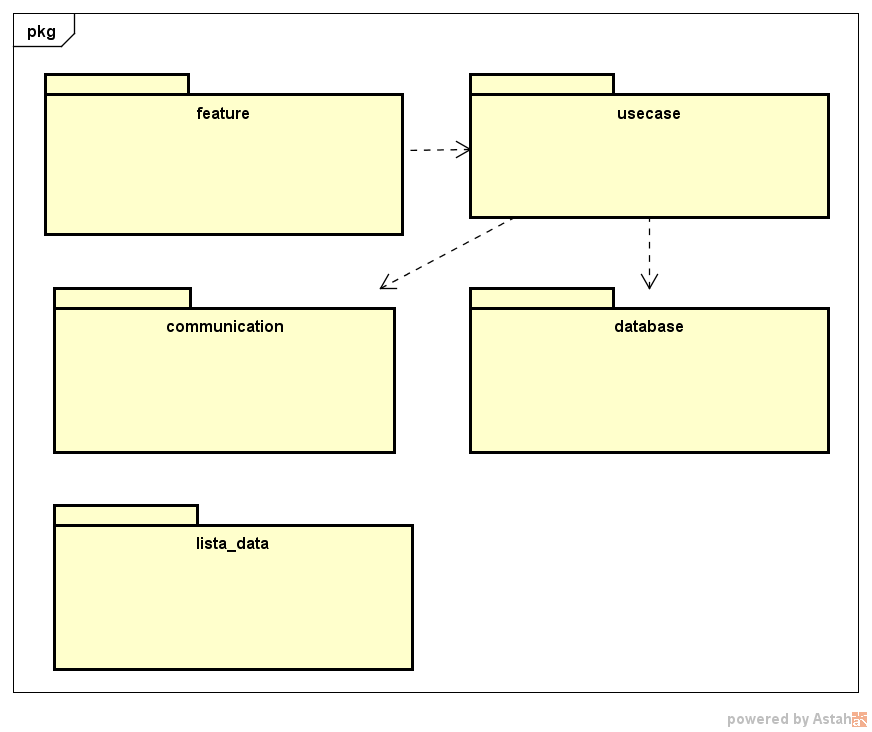
\includegraphics[scale=0.5]{Sezioni/Packages/Application/application.png}
	\caption{Package application}
\end{figure}
\begin{itemize}
	\item \textbf{Descrizione}: \termine{Package} contenente tutti i file dell'applicazione demo.
	\item \textbf{Classi e packages contenuti}:
	\begin{itemize}
		\item application::feature: package contenente tutte le feature principali dell'applicazione
		\item application::usecase: package contenente tutti gli usecase dell'applicazione
		\item application::lista\_data: package contenente le classi che modellano i dati dell'applicazione
		\item application::database: package contenente tutte le classi relative ai database
	\end{itemize}
	\item application::communication: package contenente tutte le classi atte a comunicare con la chat
\end{itemize}


\subsubsection{Package application::usecase}
\label{Package application::usecase}
\begin{figure}[H]
	\centering
	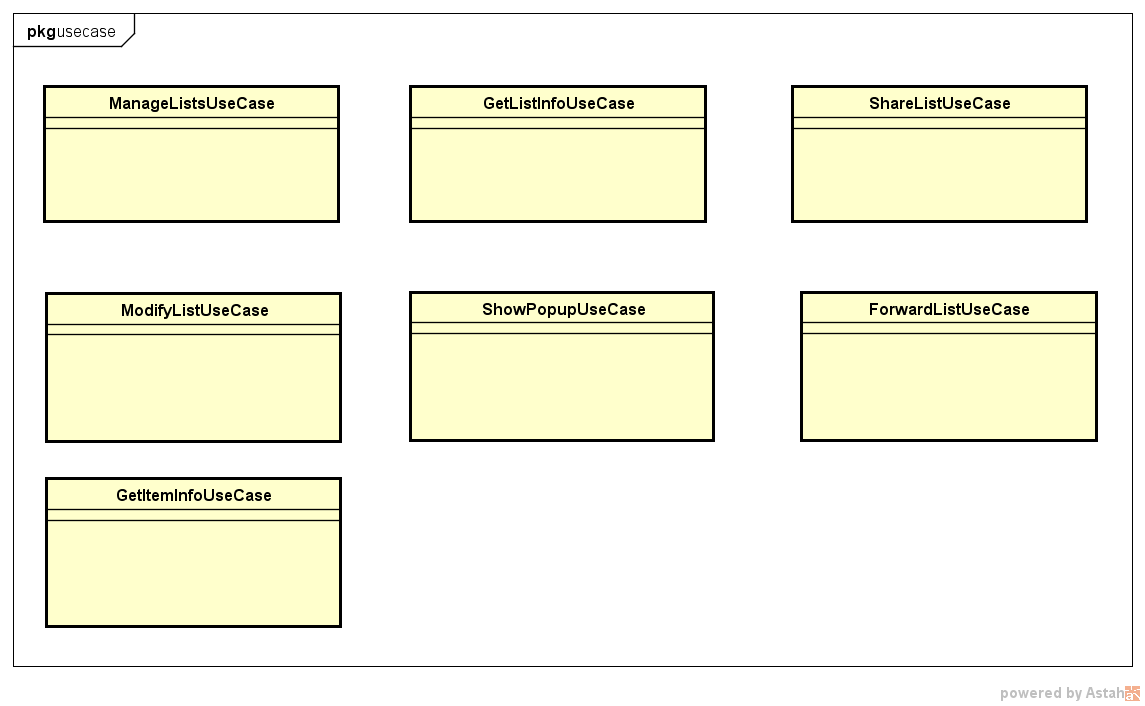
\includegraphics[scale=0.5]{Sezioni/Packages/Application/usecase.png}
	\caption{Package application::usecase}
\end{figure}
\begin{itemize}
	\item \textbf{Descrizione}: package contenente tutte le classi che gestiscono la logica dell'applicazione
	\item \textbf{Classi e packages contenuti}:
	\begin{itemize}
	\item application::usecase::ManageListsUseCase: classe che gestisce le modifiche alle liste memorizzate nel database
	\item application::usecase GetListInfoUseCase: classe che recupera i dati di una lista dal database
	\item application::usecase:ModifyListUseCase: classe che permette la modifica di una lista memorizzata all'interno del database
	\item application::usecase ShowPopupUseCase: classe che permette la visualizzazione di finestre modali
	\item application::usecase::GetItemInfoUseCase: classe che permette di recuperare le informazioni di un particolare oggetto in una lista dal database
	\end{itemize}
\end{itemize}

\subsubsection{Package application::lista\_data}
\label{Package application::lista_data}
\begin{figure}[H]
	\centering
	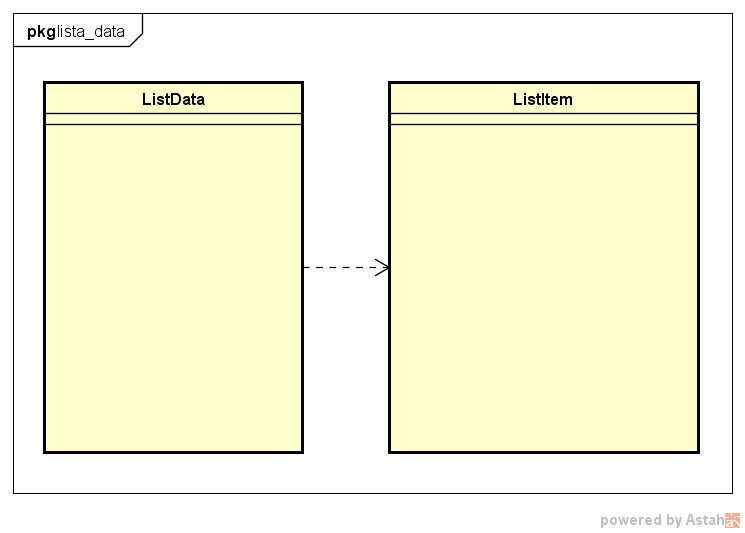
\includegraphics[scale=0.5]{Sezioni/Packages/Application/lista_data.png}
	\caption{Package application::lista\_data}
\end{figure}
\begin{itemize}
	\item \textbf{Descrizione}: package contenente tutte le classi che modellano gli oggetti di una lista e di un oggetti di una lista
	\item \textbf{Classi e packages contenuti}:
	\begin{itemize}
	\item application::lista\_data::ListData: classe che modella una lista
	\item application::lista\_data::ListItem: classe che modella un oggetto di una lista
	\end{itemize}
\end{itemize}

\subsubsection{Package application::communication}
\label{Package application::communication}
\begin{figure}[H]
	\centering
	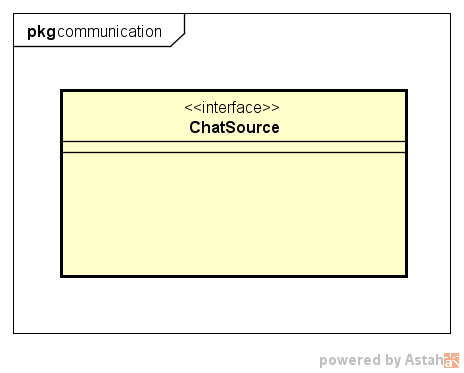
\includegraphics[scale=0.5]{Sezioni/Packages/Application/communication.png}
	\caption{Package application::communication}
\end{figure}
\begin{itemize}
	\item \textbf{Descrizione}: package che contiene le classi di comunicazione con l'istanza di Rocket.chat
	\item \textbf{Classi e packages contenuti}:
	\begin{itemize}
	\item application::communication::ChatSource: interfaccia che permette la comunicazione con l'istanza di Rocket.chat
	\end{itemize}
\end{itemize}

\subsubsection{Package application::database}
\label{Package application::database}
\begin{figure}[H]
	\centering
	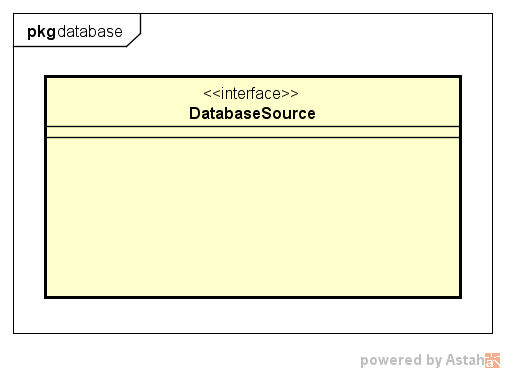
\includegraphics[scale=0.5]{Sezioni/Packages/Application/database.png}
	\caption{Package application::database}
\end{figure}
\begin{itemize}
	\item \textbf{Descrizione}: package che contiene le classi per interfacciarsi con il database all'interno del quale sono salvati i dati delle liste
	\item \textbf{Classi e packages contenuti}:
	\begin{itemize}
	\item application::database::DatabaseSource: interfaccia che permette la comunicazione con il database all'interno del quale sono salvati i dati delle varie liste
	\end{itemize}
\end{itemize}

\subsubsection{Package application::feature::add\_item}
\label{Package application::feature::add_item}
\begin{figure}[H]
	\centering
	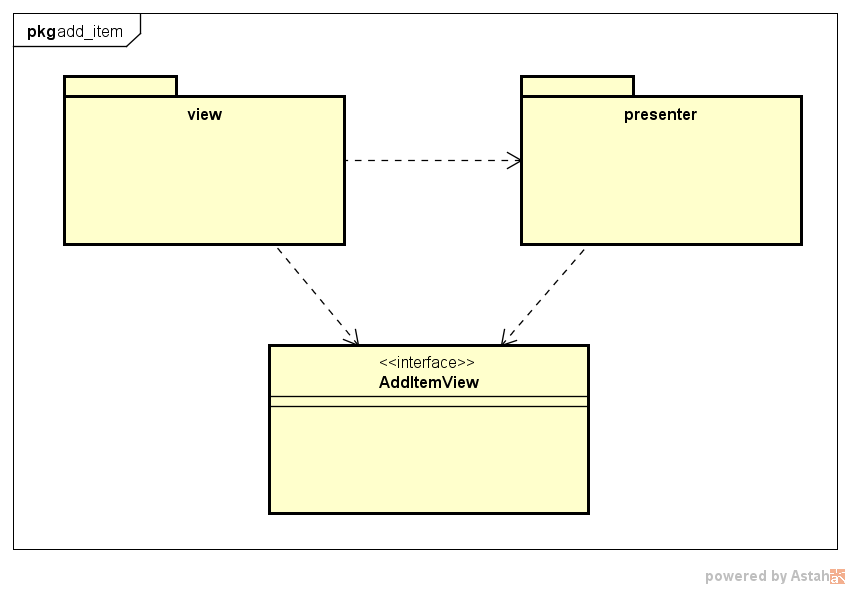
\includegraphics[scale=0.5]{Sezioni/Packages/Application/add_item.png}
	\caption{Package application::feature::add\_item}
\end{figure}
\begin{itemize}
	\item \textbf{Descrizione}: package contenente i file relativi alla funzionalità di aggiunta elemento ad una lista
	\item \textbf{Classi e packages contenuti}:
	\begin{itemize}
	\item application::feature::add\_item::view: package contenente la view per l'aggiunta di un elemento
	\item application::feature::add\_item::presenter: package contenente il presenter per la view di aggiunta elemento
	\item application::feature::add\_item::AddItemView: interfaccia che rappresenta la vista di aggiunta oggetto
	\end{itemize}
\end{itemize}

\subsubsection{Package application::feature::add\_item::view}
\label{Package application::feature::add_item::view}
\begin{figure}[H]
	\centering
	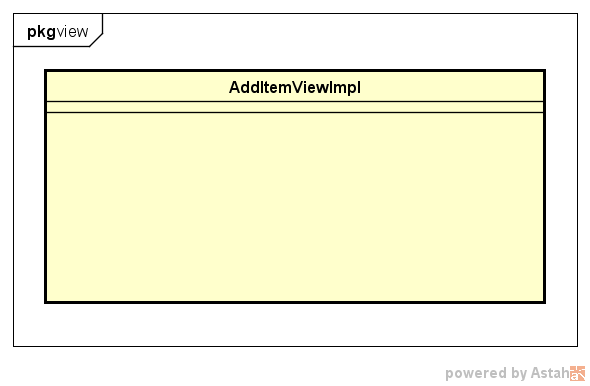
\includegraphics[scale=0.5]{Sezioni/Packages/Application/add_item_view.png}
	\caption{Package application::feature::add\_item::view}
\end{figure}
\begin{itemize}
	\item \textbf{Descrizione}: package contenente la view per l'aggiunta di un elemento
	\item \textbf{Classi e packages contenuti}:
	\begin{itemize}
	\item application::feature::add\_item::view::AddItemViewImpl: implementazione dell'interfaccia AddItemView che rappresenta la vista di aggiunta di un oggetto alla lista
	\end{itemize}
\end{itemize}

\subsubsection{Package application::feature::add\_item::presenter}
\label{Package application::feature::add_item::presenter}
\begin{figure}[H]
	\centering
	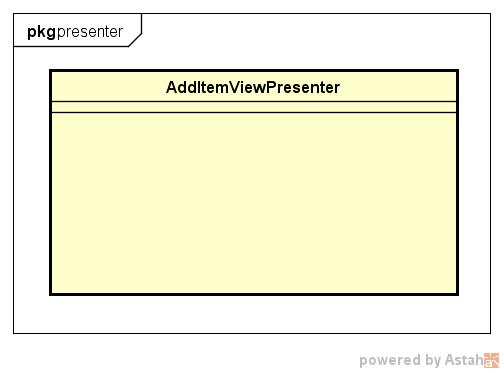
\includegraphics[scale=0.5]{Sezioni/Packages/Application/add_item_presenter.png}
	\caption{Package application::feature::add\_item::presenter}
\end{figure}
\begin{itemize}
	\item \textbf{Descrizione}: package contenente il presenter per la vista di aggiunta di un oggetto alla lista
	\item \textbf{Classi e packages contenuti}:
	\begin{itemize}
	\item application::feature::add\_item::presenter::AddItemViewPresenter: presenter per la vista di aggiunta di un oggetto alla lista
	\end{itemize}
\end{itemize}

\subsubsection{Package application::feature::change\_list\_info}
\label{Package application::feature::change_list_info}
\begin{figure}[H]
	\centering
	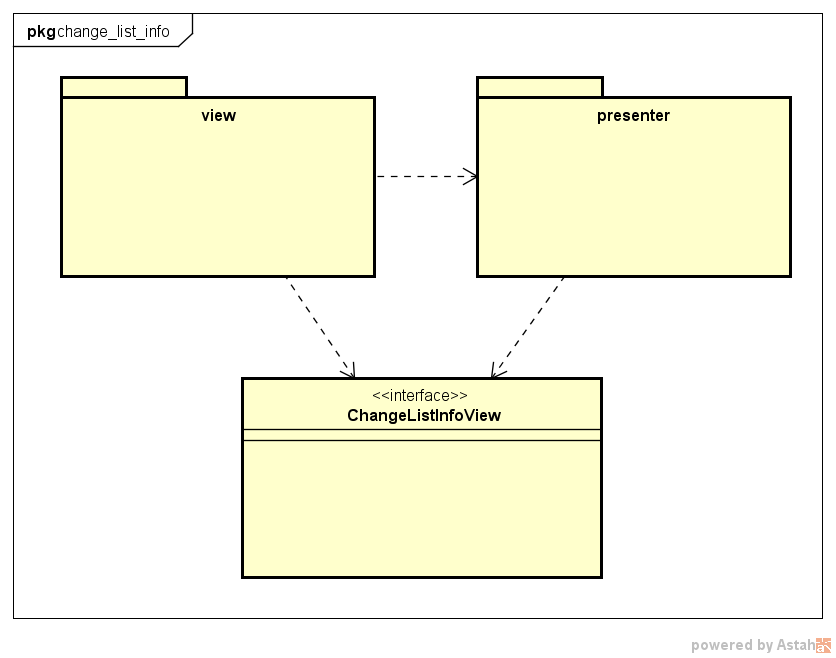
\includegraphics[scale=0.5]{Sezioni/Packages/Application/change_list_info.png}
	\caption{Package application::feature::change\_list\_info}
\end{figure}
\begin{itemize}
	\item \textbf{Descrizione}: package contenente i componenti per la funzionalità di modifica informazioni di una lista
	\item \textbf{Classi e packages contenuti}:
	\begin{itemize}
	\item application::feature::change\_list\_info::view: package contenente la vista per la modifica informazioni di una lista
	\item application::feature::change\_list\_info::presenter: package contenente il presenter per la vista di modifica informazioni di una lista
	\item application::feature::change\_list\_info::ChangeListInfoView: interfaccia rappresentante la vista per la modifica informazioni di una lista
	\end{itemize}
\end{itemize}

\subsubsection{Package application::feature::change\_list\_info::view}
\label{Package application::feature::change_list_info::view}
\begin{figure}[H]
	\centering
	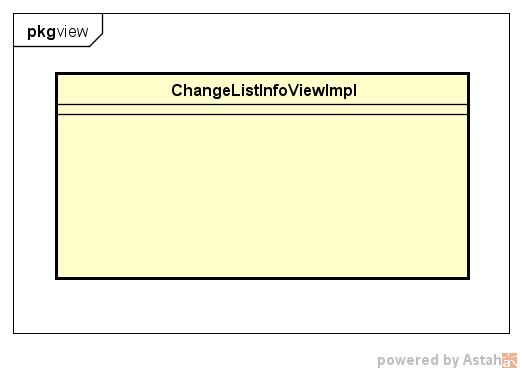
\includegraphics[scale=0.5]{Sezioni/Packages/Application/change_list_info_view.png}
	\caption{Package application::feature::change\_list\_info::view}
\end{figure}
\begin{itemize}
	\item \textbf{Descrizione}: package contenente la vista per la funzionalità di modifica informazioni di una lista
	\item \textbf{Classi e packages contenuti}:
	\begin{itemize}
	\item application::feature::change\_list\_info::view::ChangeListInfoViewImpl: implementazione dell'interfaccia che rappresenta la vista per la funzionalità di modifica della informazioni di una lista
	\end{itemize}
\end{itemize}

\subsubsection{Package application::feature::change\_list\_info::presenter}
\label{Package application::feature::change_list_info::presenter}
\begin{figure}[H]
	\centering
	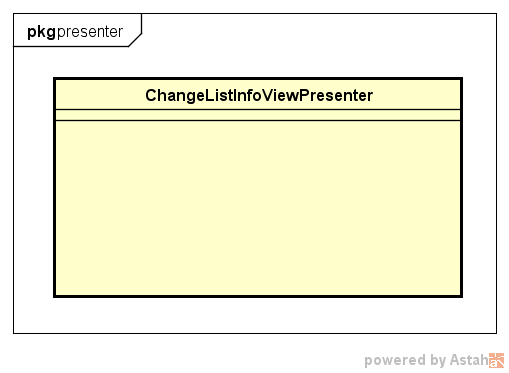
\includegraphics[scale=0.5]{Sezioni/Packages/Application/change_list_info_presenter.png}
	\caption{Package application::feature::change\_list\_info::presenter}
\end{figure}
\begin{itemize}
	\item \textbf{Descrizione}: package contenente il presenter per la vista di modifica informazioni di una lista
	\item \textbf{Classi e packages contenuti}:
	\begin{itemize}
	\item application::feature::change\_list\_info::presenter::ChangeListInfoViewPresenter: classe che rappresenta il presenter per la vista di modifica dei dati di una lista
	\end{itemize}
\end{itemize}


\subsubsection{Package application::feature::create\_list}
\label{Package application::feature::create_list}
\begin{figure}[H]
	\centering
	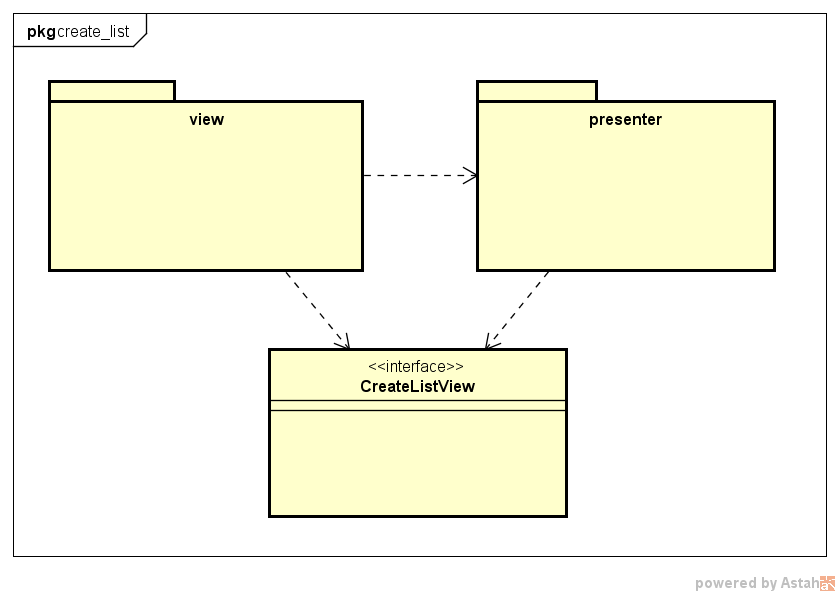
\includegraphics[scale=0.5]{Sezioni/Packages/Application/create_list.png}
	\caption{Package application::feature::create\_list}
\end{figure}
\begin{itemize}
	\item \textbf{Descrizione}: package contenente i componenti per la funzionalità di creazione di una lista
	\item \textbf{Classi e packages contenuti}:
	\begin{itemize}
	\item application::feature::create\_list::view: package contenente la vista per la creazione di una lista
	\item application::feature::create\_list::presenter: package contenente il presenter per la vista di creazione di una lista
	\item application::feature::create\_list::CreateListView: interfaccia rappresentante la vista per la creazione di una lista
	\end{itemize}
\end{itemize}

\subsubsection{Package application::feature::create\_list::view}
\label{Package application::feature::create_list::view}
\begin{figure}[H]
	\centering
	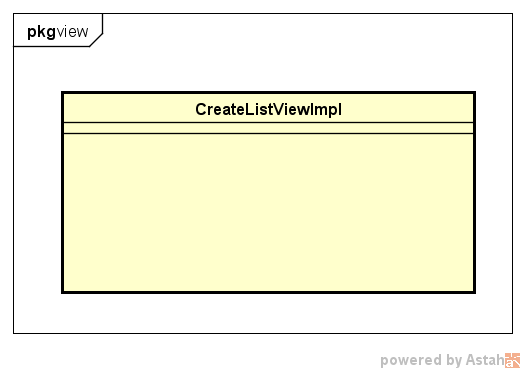
\includegraphics[scale=0.5]{Sezioni/Packages/Application/create_list_view.png}
	\caption{Package application::feature::create\_list::view}
\end{figure}
\begin{itemize}
	\item \textbf{Descrizione}: package contenente la vista per la funzionalità di creazione di una lista
	\item \textbf{Classi e packages contenuti}:
	\begin{itemize}
	\item application::feature::create\_list::view::CreateListViewImpl: implementazione dell'interfaccia che rappresenta la vista per la funzionalità di creazione di una lista
	\end{itemize}
\end{itemize}

\subsubsection{Package application::feature::create\_list::presenter}
\label{Package application::feature::create_list::presenter}
\begin{figure}[H]
	\centering
	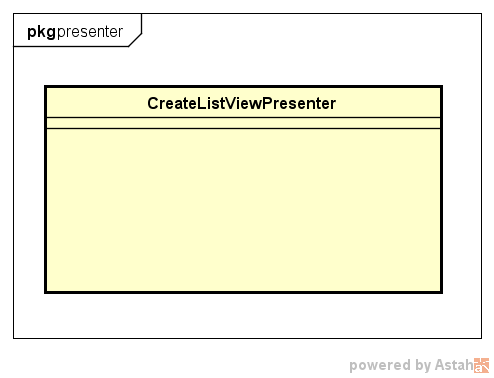
\includegraphics[scale=0.5]{Sezioni/Packages/Application/create_list_presenter.png}
	\caption{Package application::feature::create\_list::presenter}
\end{figure}
\begin{itemize}
	\item \textbf{Descrizione}: package contenente il presenter per la vista di creazione di una lista
	\item \textbf{Classi e packages contenuti}:
	\begin{itemize}
	\item application::feature::create\_list::presenter::CreateListViewPresenter: classe che rappresenta il presenter per la vista di creazione di una lista
	\end{itemize}
\end{itemize}

\subsubsection{Package application::feature::forward}
\label{Package application::feature::forward}
\begin{figure}[H]
	\centering
	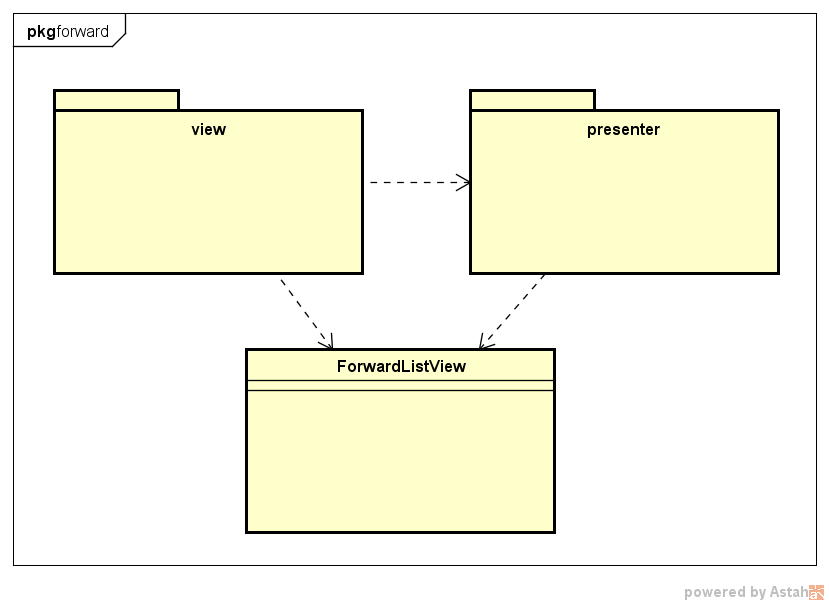
\includegraphics[scale=0.5]{Sezioni/Packages/Application/forward.png}
	\caption{Package application::feature::forward}
\end{figure}
\begin{itemize}
	\item \textbf{Descrizione}: package contenente i componenti per la funzionalità di inoltro di una lista
	\item \textbf{Classi e packages contenuti}:
	\begin{itemize}
	\item application::feature::forward::view: package contenente la vista per la inoltro di una lista
	\item application::feature::forward::presenter: package contenente il presenter per la vista di inoltro di una lista
	\item application::feature::forward::ForwardListView: interfaccia rappresentante la vista per la funzionalità inoltro di una lista
	\end{itemize}
\end{itemize}

\subsubsection{Package application::feature::forward::view}
\label{Package application::feature::forward::view}
\begin{figure}[H]
	\centering
	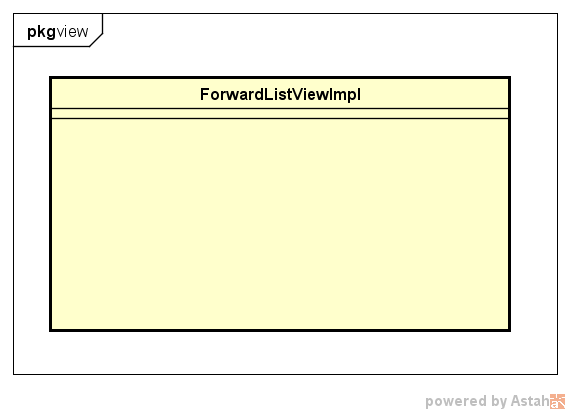
\includegraphics[scale=0.5]{Sezioni/Packages/Application/forward_view.png}
	\caption{Package application::feature::forward::view}
\end{figure}
\begin{itemize}
	\item \textbf{Descrizione}: package contenente la vista per la funzionalità di inoltro di una lista
	\item \textbf{Classi e packages contenuti}:
	\begin{itemize}
	\item application::feature::forward::view::ForwardListViewImpl: implementazione dell'interfaccia che rappresenta la vista per la funzionalità di inoltro di una lista
	\end{itemize}
\end{itemize}

\subsubsection{Package application::feature::forward::presenter}
\label{Package application::feature::forward::presenter}
\begin{figure}[H]
	\centering
	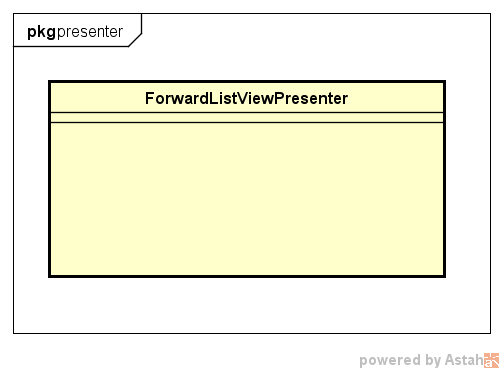
\includegraphics[scale=0.5]{Sezioni/Packages/Application/forward_presenter.png}
	\caption{Package application::feature::forward::presenter}
\end{figure}
\begin{itemize}
	\item \textbf{Descrizione}: package contenente il presenter per la vista di inoltro di una lista
	\item \textbf{Classi e packages contenuti}:
	\begin{itemize}
	\item application::feature::forward::presenter::ForwardListViewPresenter: classe che rappresenta il presenter per la vista di inoltro di una lista
	\end{itemize}
\end{itemize}

\subsubsection{Package application::feature::input\_item\_info}
\label{Package application::feature::input_item_info}
\begin{figure}[H]
	\centering
	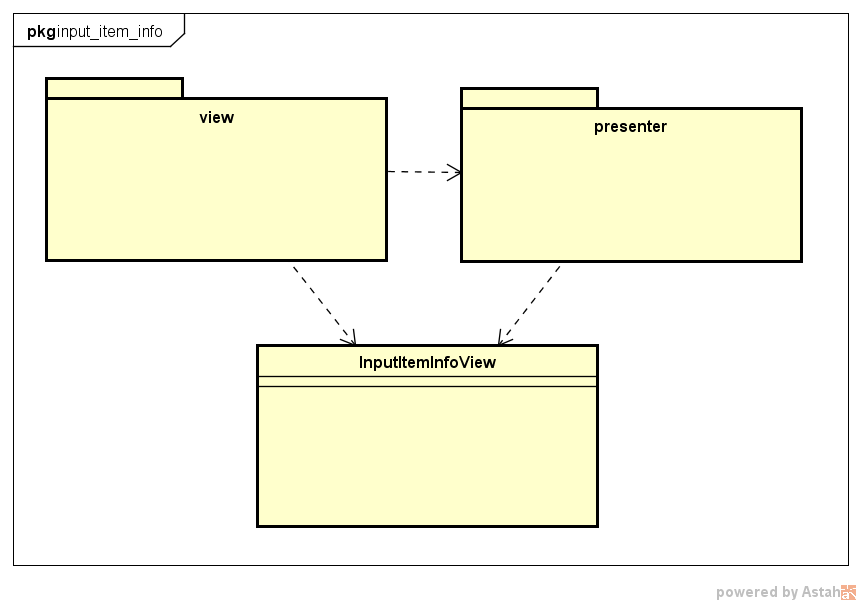
\includegraphics[scale=0.5]{Sezioni/Packages/Application/input_item_info.png}
	\caption{Package application::feature::input\_item\_info}
\end{figure}
\begin{itemize}
	\item \textbf{Descrizione}: package contenente i componenti per la funzionalità di inserimento dati di un oggetto della lista
	\item \textbf{Classi e packages contenuti}:
	\begin{itemize}
	\item application::feature::input\_item\_info::view: package contenente la vista per la inserimento dati di un oggetto della lista
	\item application::feature::input\_item\_info::presenter: package contenente il presenter per la vista di inserimento dati di un oggetto della lista
	\item application::feature::input\_item\_info::InputItemInfoView: interfaccia rappresentante la vista per la funzionalità inserimento dati di un oggetto della lista
	\end{itemize}
\end{itemize}

\subsubsection{Package application::feature::input\_item\_info::view}
\label{Package application::feature::input_item_info::view}
\begin{figure}[H]
	\centering
	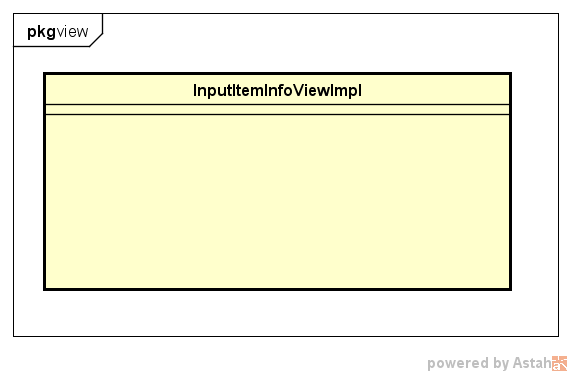
\includegraphics[scale=0.5]{Sezioni/Packages/Application/input_item_info_view.png}
	\caption{Package application::feature::input\_item\_info::view}
\end{figure}
\begin{itemize}
	\item \textbf{Descrizione}: package contenente la vista per la funzionalità di inserimento dati di un oggetto della lista
	\item \textbf{Classi e packages contenuti}:
	\begin{itemize}
	\item application::feature::input\_item\_info::view::InputItemInfoViewImpl: implementazione dell'interfaccia che rappresenta la vista per la funzionalità di inserimento dati di un oggetto della lista
	\end{itemize}
\end{itemize}

\subsubsection{Package application::feature::input\_item\_info::presenter}
\label{Package application::feature::input_item_info::presenter}
\begin{figure}[H]
	\centering
	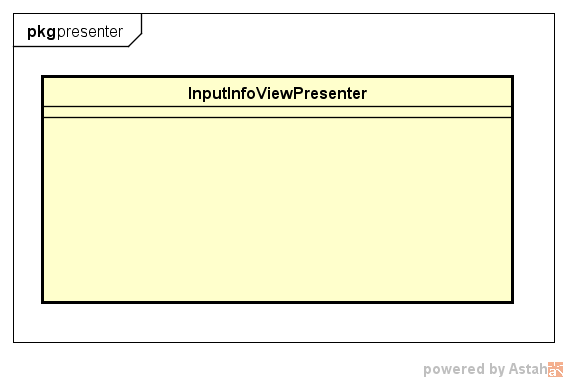
\includegraphics[scale=0.5]{Sezioni/Packages/Application/input_item_info_presenter.png}
	\caption{Package application::feature::input\_item\_info::presenter}
\end{figure}
\begin{itemize}
	\item \textbf{Descrizione}: package contenente il presenter per la vista di inserimento dati di un oggetto della lista
	\item \textbf{Classi e packages contenuti}:
	\begin{itemize}
	\item application::feature::input\_item\_info::presenter::InputItemInfoViewPresenter: classe che rappresenta il presenter per la vista di inserimento dati di un oggetto della lista
	\end{itemize}
\end{itemize}


\subsubsection{Package application::feature::input\_list\_info}
\label{Package application::feature::input_list_info}
\begin{figure}[H]
	\centering
	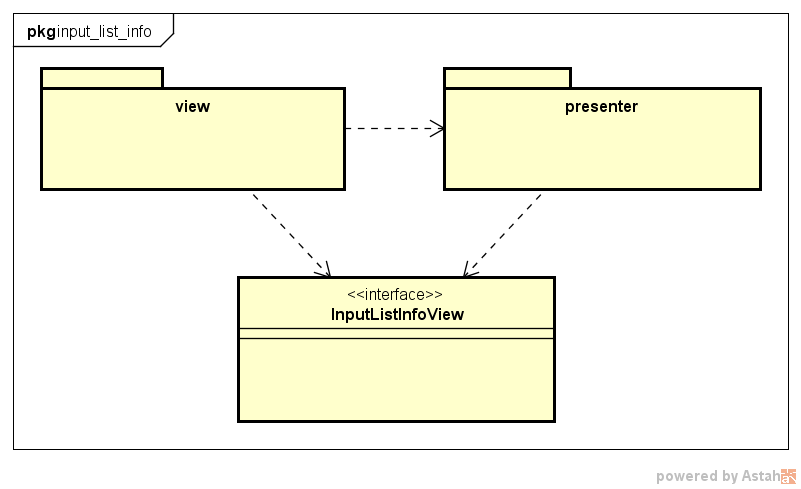
\includegraphics[scale=0.5]{Sezioni/Packages/Application/input_list_info.png}
	\caption{Package application::feature::input\_list\_info}
\end{figure}
\begin{itemize}
	\item \textbf{Descrizione}: package contenente i componenti per la funzionalità di inserimento dati di una lista
	\item \textbf{Classi e packages contenuti}:
	\begin{itemize}
	\item application::feature::input\_list\_info::view: package contenente la vista per la inserimento dati di una lista
	\item application::feature::input\_list\_info::presenter: package contenente il presenter per la vista di inserimento dati di una lista
	\item application::feature::input\_list\_info::InputListInfoView: interfaccia rappresentante la vista per la funzionalità inserimento dati di una lista
	\end{itemize}
\end{itemize}

\subsubsection{Package application::feature::input\_list\_info::view}
\label{Package application::feature::input_list_info::view}
\begin{figure}[H]
	\centering
	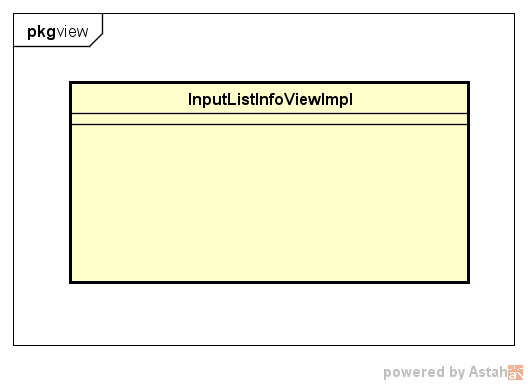
\includegraphics[scale=0.5]{Sezioni/Packages/Application/input_list_info_view.png}
	\caption{Package application::feature::input\_list\_info::view}
\end{figure}
\begin{itemize}
	\item \textbf{Descrizione}: package contenente la vista per la funzionalità di inserimento dati di una lista
	\item \textbf{Classi e packages contenuti}:
	\begin{itemize}
	\item application::feature::input\_list\_info::view::InputListInfoViewImpl: implementazione dell'interfaccia che rappresenta la vista per la funzionalità di inserimento dati di una lista
	\end{itemize}
\end{itemize}

\subsubsection{Package application::feature::input\_list\_info::presenter}
\label{Package application::feature::input_list_info::presenter}
\begin{figure}[H]
	\centering
	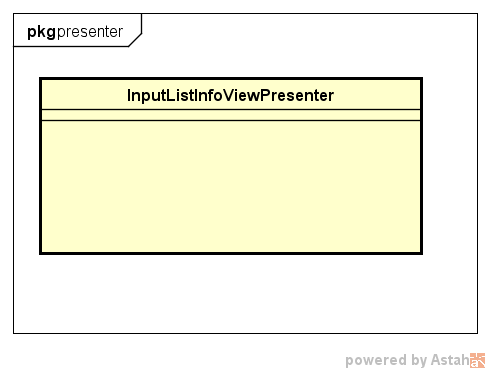
\includegraphics[scale=0.5]{Sezioni/Packages/Application/input_list_info_presenter.png}
	\caption{Package application::feature::input\_list\_info::presenter}
\end{figure}
\begin{itemize}
	\item \textbf{Descrizione}: package contenente il presenter per la vista di inserimento dati di una lista
	\item \textbf{Classi e packages contenuti}:
	\begin{itemize}
	\item application::feature::input\_list\_info::presenter::InputListInfoViewPresenter: classe che rappresenta il presenter per la vista di inserimento dati di una lista
	\end{itemize}
\end{itemize}


\subsubsection{Package application::feature::modify\_item}
\label{Package application::feature::modify_item}
\begin{figure}[H]
	\centering
	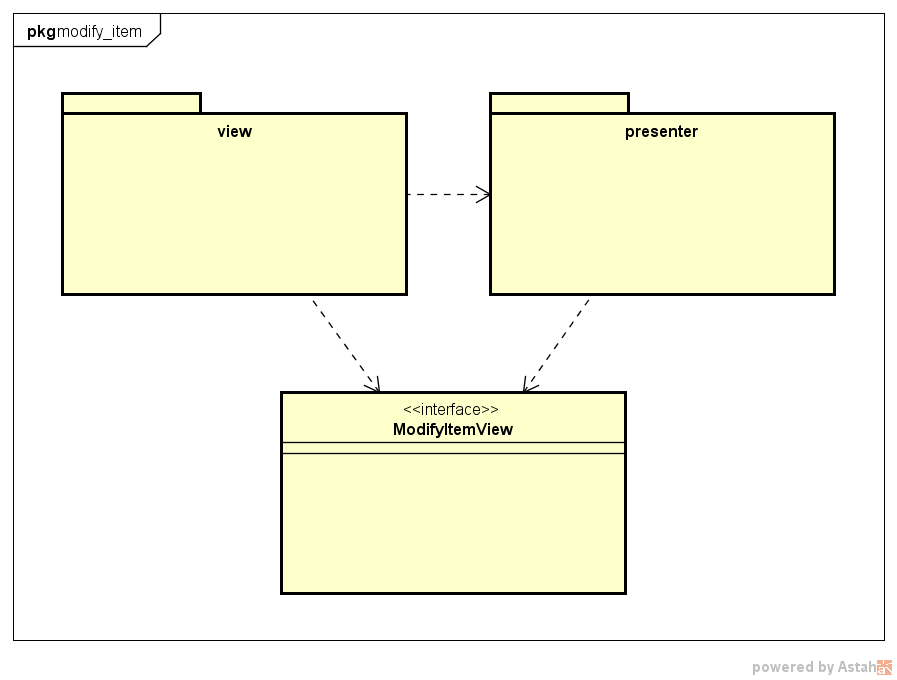
\includegraphics[scale=0.5]{Sezioni/Packages/Application/modify_item.png}
	\caption{Package application::feature::modify\_item}
\end{figure}
\begin{itemize}
	\item \textbf{Descrizione}: package contenente i componenti per la funzionalità di modifica di un oggetto all'interno di una lista
	\item \textbf{Classi e packages contenuti}:
	\begin{itemize}
	\item application::feature::modify\_item::view: package contenente la vista per la modifica di un oggetto all'interno di una lista
	\item application::feature::modify\_item::presenter: package contenente il presenter per la vista di modifica di un oggetto all'interno di una lista
	\item application::feature::modify\_item::ModifyItemView: interfaccia rappresentante la vista per la funzionalità modifica di un oggetto all'interno di una lista
	\end{itemize}
\end{itemize}

\subsubsection{Package application::feature::modify\_item::view}
\label{Package application::feature::modify_item::view}
\begin{figure}[H]
	\centering
	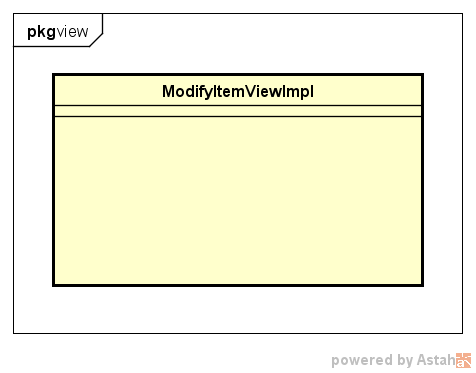
\includegraphics[scale=0.5]{Sezioni/Packages/Application/modify_item_view.png}
	\caption{Package application::feature::modify\_item::view}
\end{figure}
\begin{itemize}
	\item \textbf{Descrizione}: package contenente la vista per la funzionalità di modifica di un oggetto all'interno di una lista
	\item \textbf{Classi e packages contenuti}:
	\begin{itemize}
	\item application::feature::modify\_item::view::ModifyItemViewImpl: implementazione dell'interfaccia che rappresenta la vista per la funzionalità di modifica di un oggetto all'interno di una lista
	\end{itemize}
\end{itemize}

\subsubsection{Package application::feature::modify\_item::presenter}
\label{Package application::feature::modify_item::presenter}
\begin{figure}[H]
	\centering
	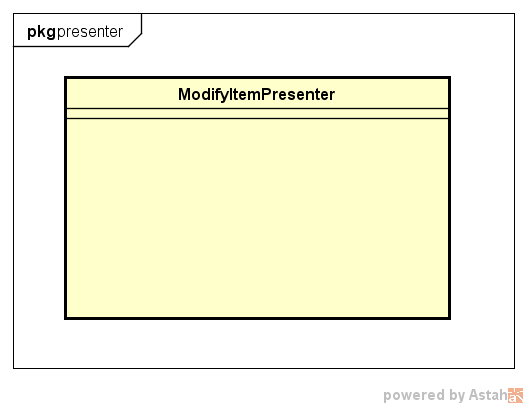
\includegraphics[scale=0.5]{Sezioni/Packages/Application/modify_item_presenter.png}
	\caption{Package application::feature::modify\_item::presenter}
\end{figure}
\begin{itemize}
	\item \textbf{Descrizione}: package contenente il presenter per la vista di modifica di un oggetto all'interno di una lista
	\item \textbf{Classi e packages contenuti}:
	\begin{itemize}
	\item application::feature::modify\_item::presenter::ModifyItemViewPresenter: classe che rappresenta il presenter per la vista di modifica di un oggetto all'interno di una lista
	\end{itemize}
\end{itemize}


\subsubsection{Package application::feature::remove\_item}
\label{Package application::feature::remove_item}
\begin{figure}[H]
	\centering
	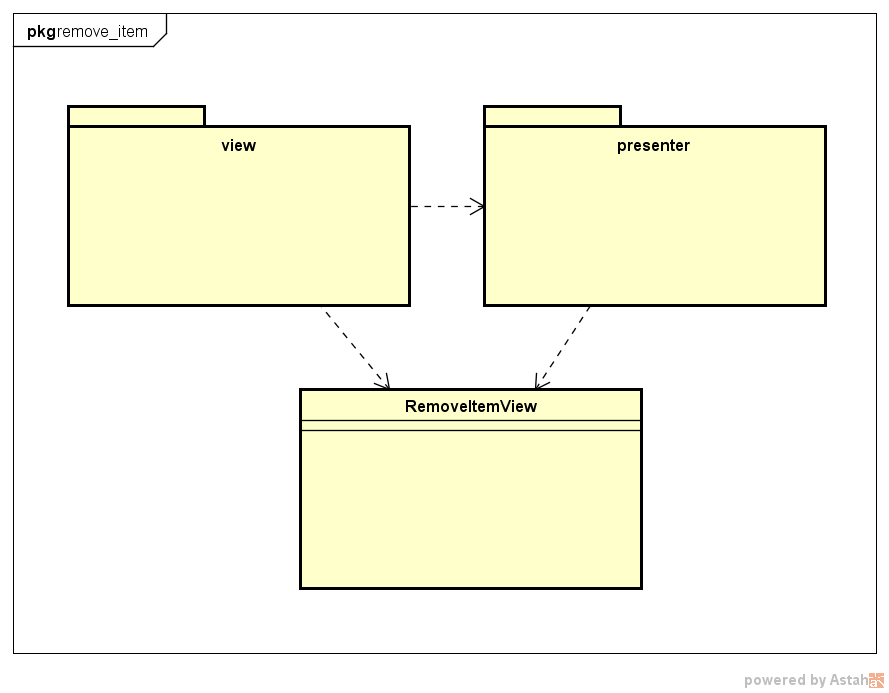
\includegraphics[scale=0.5]{Sezioni/Packages/Application/remove_item.png}
	\caption{Package application::feature::remove\_item}
\end{figure}
\begin{itemize}
	\item \textbf{Descrizione}: package contenente i componenti per la funzionalità di rimozione di un oggetto da una lista
	\item \textbf{Classi e packages contenuti}:
	\begin{itemize}
	\item application::feature::remove\_item::view: package contenente la vista per la modifica di un oggetto all'interno di una lista
	\item application::feature::remove\_item::presenter: package contenente il presenter per la vista di modifica di un oggetto all'interno di una lista
	\item application::feature::remove\_item::RemoveItemView: interfaccia rappresentante la vista per la funzionalità modifica di un oggetto all'interno di una lista
	\end{itemize}
\end{itemize}

\subsubsection{Package application::feature::remove\_item::view}
\label{Package application::feature::remove_item::view}
\begin{figure}[H]
	\centering
	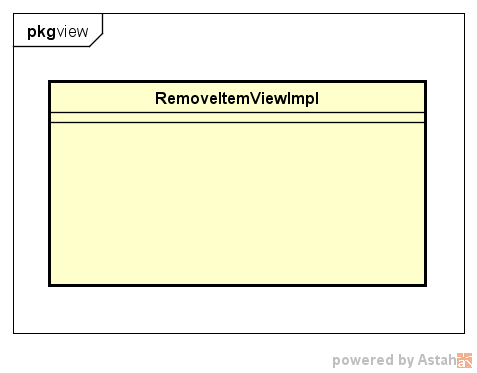
\includegraphics[scale=0.5]{Sezioni/Packages/Application/remove_item_view.png}
	\caption{Package application::feature::remove\_item::view}
\end{figure}
\begin{itemize}
	\item \textbf{Descrizione}: package contenente la vista per la funzionalità di rimozione di un oggetto da una lista
	\item \textbf{Classi e packages contenuti}:
	\begin{itemize}
	\item application::feature::remove\_item::view::RemoveItemViewImpl: implementazione dell'interfaccia che rappresenta la vista per la funzionalità di rimozione di un oggetto da una lista
	\end{itemize}
\end{itemize}

\subsubsection{Package application::feature::remove\_item::presenter}
\label{Package application::feature::remove_item::presenter}
\begin{figure}[H]
	\centering
	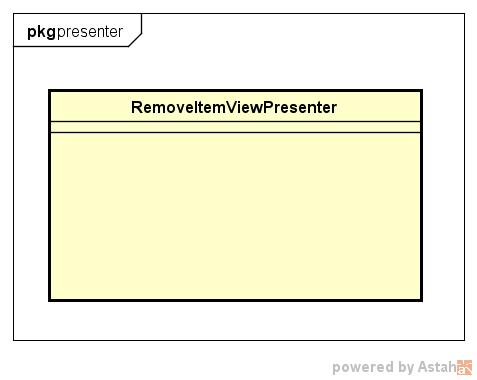
\includegraphics[scale=0.5]{Sezioni/Packages/Application/remove_item_presenter.png}
	\caption{Package application::feature::forward::remove\_item::presenter}
\end{figure}
\begin{itemize}
	\item \textbf{Descrizione}: package contenente il presenter per la vista di rimozione di un oggetto da una lista
	\item \textbf{Classi e packages contenuti}:
	\begin{itemize}
	\item application::feature::remove\_item::presenter::RemoveItemViewPresenter: classe che rappresenta il presenter per la vista di rimozione di un oggetto da una lista
	\end{itemize}
\end{itemize}


\subsubsection{Package application::feature::sharewithcontact}
\label{Package application::feature::sharewithcontact}
\begin{figure}[H]
	\centering
	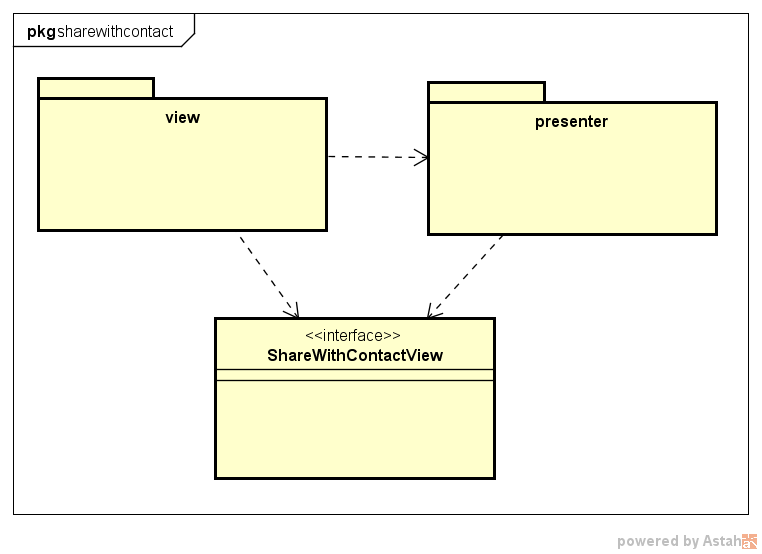
\includegraphics[scale=0.5]{Sezioni/Packages/Application/share_with_contact.png}
	\caption{Package application::feature::sharewithcontact}
\end{figure}
\begin{itemize}
	\item \textbf{Descrizione}: package contenente i componenti per la funzionalità di condivisione della lista con un contatto
	\item \textbf{Classi e packages contenuti}:
	\begin{itemize}
	\item application::feature::sharewithcontact::view: package contenente la vista per la modifica di un oggetto all'interno di una lista
	\item application::feature::sharewithcontact::presenter: package contenente il presenter per la vista di modifica di un oggetto all'interno di una lista
	\item application::feature::sharewithcontact::ShareWithContactView: interfaccia rappresentante la vista per la funzionalità modifica di un oggetto all'interno di una lista
	\end{itemize}
\end{itemize}

\subsubsection{Package application::feature::sharewithcontact::view}\label{Package application::feature::sharewithcontact::view}
\begin{figure}[H]
	\centering
	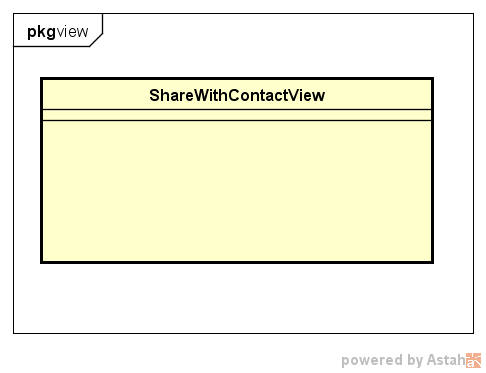
\includegraphics[scale=0.5]{Sezioni/Packages/Application/share_with_contact_view.png}
	\caption{Package application::feature::sharewithcontact::view}
\end{figure}
\begin{itemize}
	\item \textbf{Descrizione}: package contenente la vista per la funzionalità di condivisione della lista con un contatto
	\item \textbf{Classi e packages contenuti}:
	\begin{itemize}
	\item application::feature::sharewithcontact::view::ShareWithContactViewImpl: implementazione dell'interfaccia che rappresenta la vista per la funzionalità di condivisione della lista con un contatto
	\end{itemize}
\end{itemize}

\subsubsection{Package application::feature::sharewithcontact::presenter}
\label{Package application::feature::sharewithcontact::presenter}
\begin{figure}[H]
	\centering
	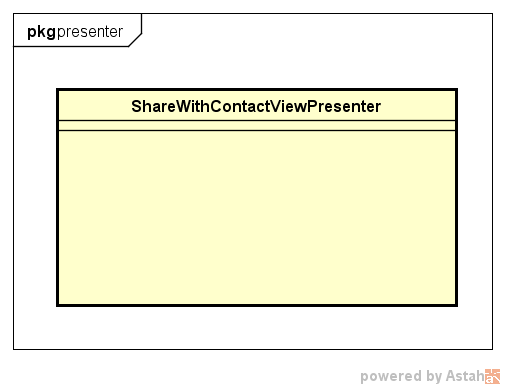
\includegraphics[scale=0.5]{Sezioni/Packages/Application/share_with_contact_presenter.png}
	\caption{Package application::feature::sharewithcontact::presenter}
\end{figure}
\begin{itemize}
	\item \textbf{Descrizione}: package contenente il presenter per la vista di condivisione della lista con un contatto
	\item \textbf{Classi e packages contenuti}:
	\begin{itemize}
	\item application::feature::sharewithcontact::presenter::ShareWithContactViewPresenter: classe che rappresenta il presenter per la vista di condivisione della lista con un contatto
	\end{itemize}
\end{itemize}


\subsubsection{Package application::feature::sharewithgroup}
\label{Package application::feature::sharewithgroup}
\begin{figure}[H]
	\centering
	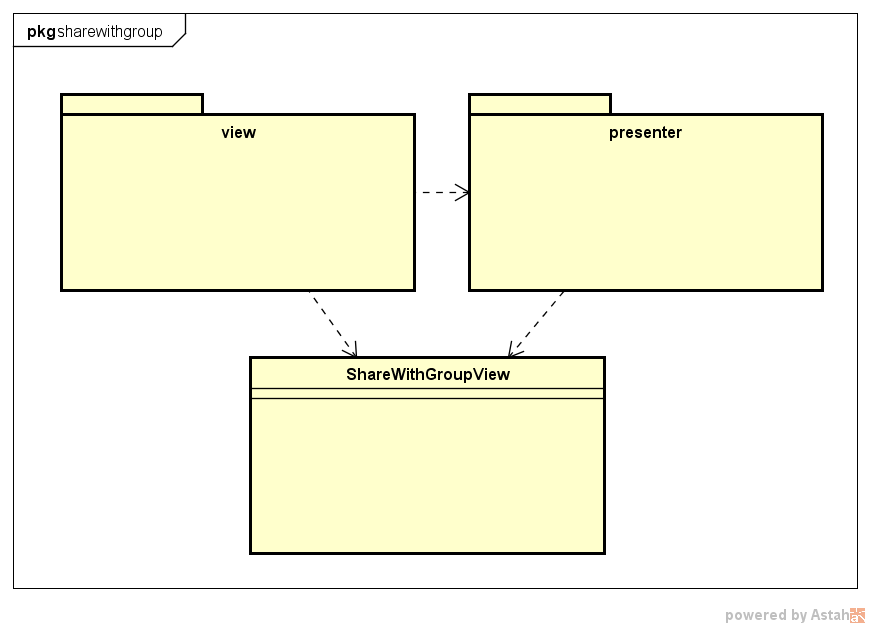
\includegraphics[scale=0.5]{Sezioni/Packages/Application/share_with_group.png}
	\caption{Package application::feature::sharewithgroup}
\end{figure}
\begin{itemize}
	\item \textbf{Descrizione}: package contenente i componenti per la funzionalità di condivisione della lista con un gruppo
	\item \textbf{Classi e packages contenuti}:
	\begin{itemize}
	\item application::feature::sharewithgroup::view: package contenente la vista per la modifica di un oggetto all'interno di una lista
	\item application::feature::sharewithgroup::presenter: package contenente il presenter per la vista di modifica di un oggetto all'interno di una lista
	\item application::feature::sharewithgroup::ShareWithGroupView: interfaccia rappresentante la vista per la funzionalità modifica di un oggetto all'interno di una lista
	\end{itemize}
\end{itemize}

\subsubsection{Package application::feature::sharewithgroup::view}
\label{Package application::feature::sharewithgroup::view}
\begin{figure}[H]
	\centering
	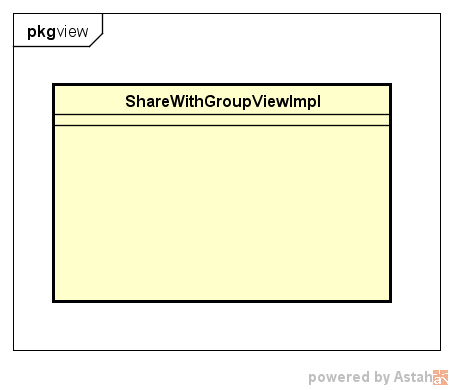
\includegraphics[scale=0.5]{Sezioni/Packages/Application/share_with_group_view.png}
	\caption{Package application::feature::sharewithgroup::view}
\end{figure}
\begin{itemize}
	\item \textbf{Descrizione}: package contenente la vista per la funzionalità di condivisione della lista con un gruppo
	\item \textbf{Classi e packages contenuti}:
	\begin{itemize}
	\item application::feature::sharewithgroup::view::ShareWithGroupViewImpl: implementazione dell'interfaccia che rappresenta la vista per la funzionalità di condivisione della lista con un gruppo
	\end{itemize}
\end{itemize}

\subsubsection{Package application::feature::sharewithgroup::presenter}
\label{Package application::feature::sharewithgroup::presenter}
\begin{figure}[H]
	\centering
	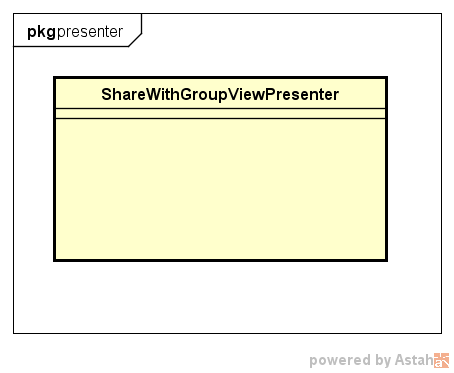
\includegraphics[scale=0.5]{Sezioni/Packages/Application/share_with_group_presenter.png}
	\caption{Package application::feature::sharewithgroup::presenter}
\end{figure}
\begin{itemize}
	\item \textbf{Descrizione}: package contenente il presenter per la vista di condivisione della lista con un gruppo
	\item \textbf{Classi e packages contenuti}:
	\begin{itemize}
	\item application::feature::sharewithgroup::presenter::ShareWithGroupViewPresenter: classe che rappresenta il presenter per la vista di condivisione della lista con un gruppo
	\end{itemize}
\end{itemize}


\subsubsection{Package application::feature::help}
\label{Package application::feature::help}
\begin{figure}[H]
	\centering
	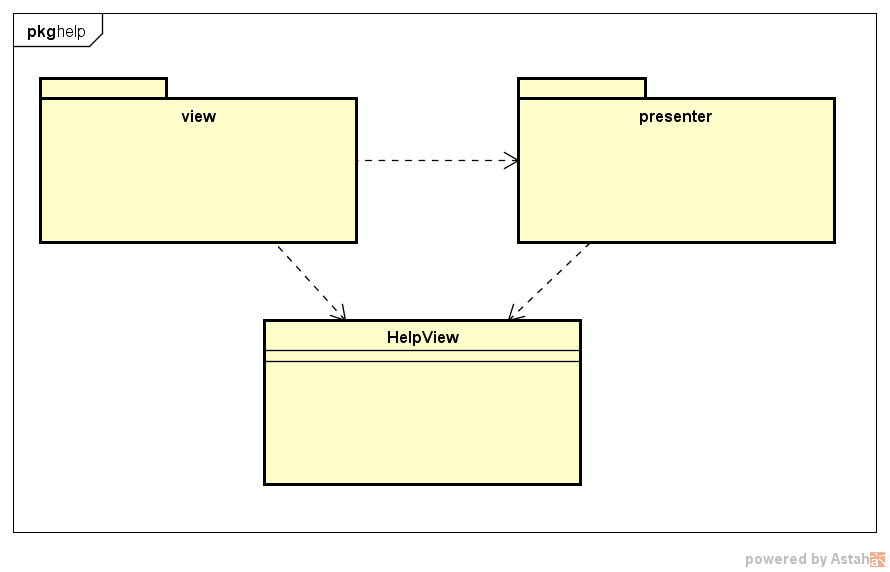
\includegraphics[scale=0.5]{Sezioni/Packages/Application/help.png}
	\caption{Package application::feature::help}
\end{figure}
\begin{itemize}
	\item \textbf{Descrizione}: package contenente i componenti per la funzionalità di visualizzazione aiuto per l'utilizzo dell'applicazione
	\item \textbf{Classi e packages contenuti}:
	\begin{itemize}
	\item application::feature::help::view: package contenente la vista per la modifica di un oggetto all'interno di una lista
	\item application::feature::help::presenter: package contenente il presenter per la vista di modifica di un oggetto all'interno di una lista
	\item application::feature::help::helpView: interfaccia rappresentante la vista per la funzionalità modifica di un oggetto all'interno di una lista
	\end{itemize}
\end{itemize}

\subsubsection{Package application::feature::help::view}
\label{Package application::feature::help::view}
\begin{figure}[H]
	\centering
	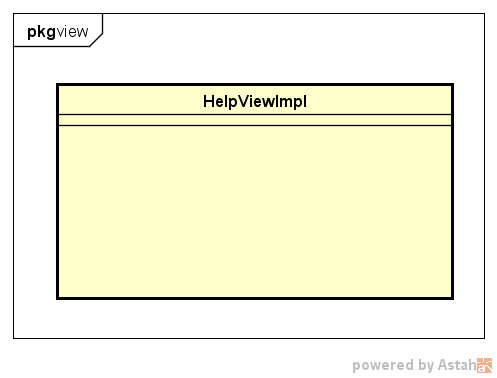
\includegraphics[scale=0.5]{Sezioni/Packages/Application/help_view.png}
	\caption{Package application::feature::help::view}
\end{figure}
\begin{itemize}
	\item \textbf{Descrizione}: package contenente la vista per la funzionalità di visualizzazione aiuto per l'utilizzo dell'applicazione
	\item \textbf{Classi e packages contenuti}:
	\begin{itemize}
	\item application::feature::help::view::helpViewImpl: implementazione dell'interfaccia che rappresenta la vista per la funzionalità di visualizzazione aiuto per l'utilizzo dell'applicazione
	\end{itemize}
\end{itemize}

\subsubsection{Package application::feature::help::presenter}
\label{Package application::feature::help::presenter}
\begin{figure}[H]
	\centering
	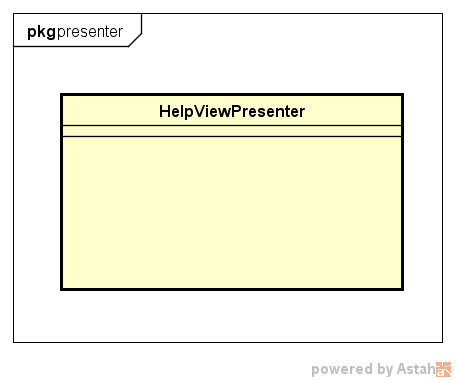
\includegraphics[scale=0.5]{Sezioni/Packages/Application/help_presenter.png}
	\caption{Package application::feature::help::presenter}
\end{figure}
\begin{itemize}
	\item \textbf{Descrizione}: package contenente il presenter per la vista di visualizzazione aiuto per l'utilizzo dell'applicazione
	\item \textbf{Classi e packages contenuti}:
	\begin{itemize}
	\item application::feature::help::presenter::helpViewPresenter: classe che rappresenta il presenter per la vista di visualizzazione aiuto per l'utilizzo dell'applicazione
	\end{itemize}
\end{itemize}

\subsubsection{Package application::feature::exception}
\label{Package application::feature::exception}
\begin{figure}[H]
	\centering
	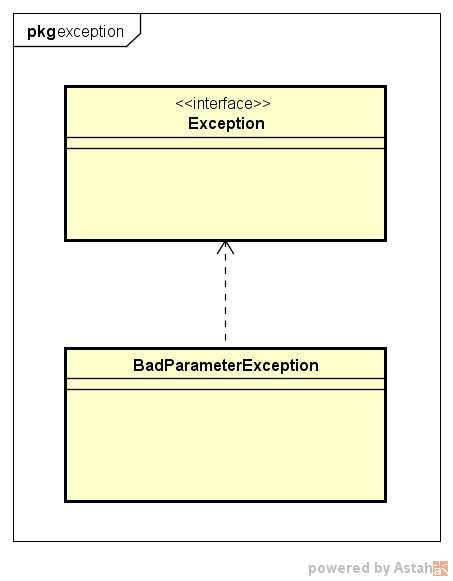
\includegraphics[scale=0.5]{Sezioni/Packages/Application/exception.png}
	\caption{Package application::feature::exception}
\end{figure}
\begin{itemize}
	\item \textbf{Descrizione}: package contenente tutte le eccezioni che l'applicazione può lanciare durante l'esecuzione
	\item \textbf{Classi e packages contenuti}:
	\begin{itemize}
	\item application::feature::exception::Exception: classe che rappresenta una eccezione generica
	\item application::feature::exception::BadParameterException: classe che rappresenta una eccezione lanciata nel qual caso un parametro di un metodo sia incorretto
	\end{itemize}
\end{itemize}
